% Options for packages loaded elsewhere
\PassOptionsToPackage{unicode}{hyperref}
\PassOptionsToPackage{hyphens}{url}
%
\documentclass[10pt,a4paper]{article}
\usepackage[left=25mm,right=25mm]{geometry}
\usepackage{amsmath}
\usepackage{amsfonts}
\usepackage{amssymb}

\usepackage{amsmath,amssymb}
\usepackage{lmodern}
\usepackage{iftex}
\ifPDFTeX
  \usepackage[T1]{fontenc}
  \usepackage[utf8]{inputenc}
  \usepackage{textcomp} % provide euro and other symbols
\else % if luatex or xetex
  \usepackage{unicode-math}
  \defaultfontfeatures{Scale=MatchLowercase}
  \defaultfontfeatures[\rmfamily]{Ligatures=TeX,Scale=1}
\fi
% Use upquote if available, for straight quotes in verbatim environments
\IfFileExists{upquote.sty}{\usepackage{upquote}}{}
\IfFileExists{microtype.sty}{% use microtype if available
  \usepackage[]{microtype}
  \UseMicrotypeSet[protrusion]{basicmath} % disable protrusion for tt fonts
}{}
\makeatletter
\@ifundefined{KOMAClassName}{% if non-KOMA class
  \IfFileExists{parskip.sty}{%
    \usepackage{parskip}
  }{% else
    \setlength{\parindent}{0pt}
    \setlength{\parskip}{6pt plus 2pt minus 1pt}}
}{% if KOMA class
  \KOMAoptions{parskip=half}}
\makeatother
\usepackage{xcolor}
\usepackage{longtable,booktabs,array}
\usepackage{multirow}
\usepackage{calc} % for calculating minipage widths
% Correct order of tables after \paragraph or \subparagraph
\usepackage{etoolbox}
\makeatletter
\patchcmd\longtable{\par}{\if@noskipsec\mbox{}\fi\par}{}{}
\makeatother
% Allow footnotes in longtable head/foot
\IfFileExists{footnotehyper.sty}{\usepackage{footnotehyper}}{\usepackage{footnote}}
\makesavenoteenv{longtable}
\usepackage{graphicx}
\makeatletter
\def\maxwidth{\ifdim\Gin@nat@width>\linewidth\linewidth\else\Gin@nat@width\fi}
\def\maxheight{\ifdim\Gin@nat@height>\textheight\textheight\else\Gin@nat@height\fi}
\makeatother
% Scale images if necessary, so that they will not overflow the page
% margins by default, and it is still possible to overwrite the defaults
% using explicit options in \includegraphics[width, height, ...]{}
\setkeys{Gin}{width=\maxwidth,height=\maxheight,keepaspectratio}
% Set default figure placement to htbp
\makeatletter
\def\fps@figure{htbp}
\makeatother
\setlength{\emergencystretch}{3em} % prevent overfull lines
\providecommand{\tightlist}{%
  \setlength{\itemsep}{0pt}\setlength{\parskip}{0pt}}
\setcounter{secnumdepth}{-\maxdimen} % remove section numbering
\ifLuaTeX
  \usepackage{selnolig}  % disable illegal ligatures
\fi
\IfFileExists{bookmark.sty}{\usepackage{bookmark}}{\usepackage{hyperref}}
\IfFileExists{xurl.sty}{\usepackage{xurl}}{} % add URL line breaks if available
\urlstyle{same} % disable monospaced font for URLs
\hypersetup{
  hidelinks,
  pdfcreator={LaTeX via pandoc}}

\author{}
\date{}



\usepackage{listings}
\usepackage{color}

\definecolor{dkgreen}{rgb}{0,0.6,0}
\definecolor{gray}{rgb}{0.5,0.5,0.5}
\definecolor{mauve}{rgb}{0.58,0,0.82}

\lstset{frame=tb,
  language=C,
  aboveskip=3mm,
  belowskip=3mm,
  showstringspaces=false,
  columns=flexible,
  basicstyle={\small\ttfamily},
  numbers=none,
  numberstyle=\tiny\color{gray},
  keywordstyle=\color{blue},
  commentstyle=\color{dkgreen},
  stringstyle=\color{mauve},
  breaklines=true,
  breakatwhitespace=true,
  tabsize=3
}

\usepackage{multicol}
\usepackage{graphicx}
\usepackage{epstopdf}

\epstopdfDeclareGraphicsRule{.gif}{png}{.png}{convert gif:#1 png:\OutputFile}
\AppendGraphicsExtensions{.gif}
\usepackage{chngcntr}
\counterwithin*{equation}{section}
\counterwithin*{equation}{subsection}

\usepackage{float} 

\usepackage{amsmath}
\let\oldsubsection\subsection
\renewcommand{\subsection}{%
    \setcounter{equation}{0}%
    \oldsubsection%
}

\begin{document}


\begin{flushleft}
\begin{LARGE}CPRE 488 Homework 2 Spring 2024
\end{LARGE}
\\Digital Camera Sensor
\\Jonathan Hess
\\\href{https://github.com/Jetsama/CPRE488/tree/main/HW2}{GitHub Page}
\end{flushleft}

\section{Problem 1}
\begin{quote}
CPU Architecture. Why are ARM processors significantly more prevalent in modern embedded systems than
comparable processors from Intel (e.g. Intel Atom-based products)? Provide at least two reasons. What are
three meaningful differences between the ARMv8 ISA and x86-64? Be specific.
\end{quote}

Arm processors do not have to support the entire x86-64 instruction set. The x86-64 is backwards comparable (because porting programs between instruction sets used to be expensive). This means that the instructions set of ARM (RISC: Reduced Instruction Set Computing) is fewer and takes less power. The ARM process is designed for efficiency rather than speed which is optimal for low power control embedded systems.

\section{Problem 2}
\begin{quote}
Digital Camera Sensors. A digital camera uses an array of photo-sensors to capture an image. When the
shutter button is pressed, the exposure process begins, and light is directed through a lens to the individual
sensors, each of which measures the resulting intensity. The relative quantity of photons at each sensor site are
read as electrical signals and collected as digital values, the precision of which is determined by the bit depth.
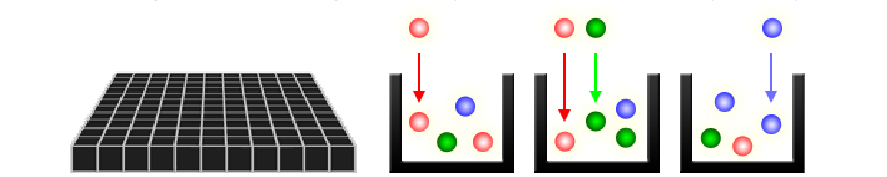
\includegraphics[width=3in]{images/Problem2-1.png} \\

However, the photosites illustrated above would only be able to capture grayscale images, since the sensors are
unable to distinguish between the red, green, and blue intensities of the luminous exposure. To capture color
images, a filter has to be placed over each cavity that permits only particular wavelengths of light. Most digital
cameras only capture one of the three primary colors at each site, and so they discard (roughly) two-thirds of
the incoming light. Consequently, the camera has to approximate the other two primary colors in order to have
a full color for each pixel. The most common type of color filter array is called a “Bayer array”, as is shown
below.

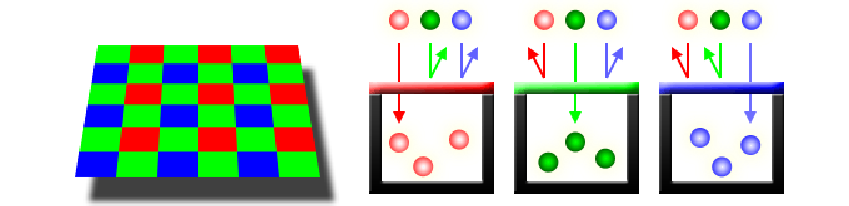
\includegraphics[width=3in]{images/Problem2-2.png} \\

\end{quote}



\subsection{Problem 2a}
\begin{quote}
The Bayer filter uses a simple strategy: capture alternating red, green, and blue colors at each sensor, with twice
as many green filters as red and blue. Briefly explain why more green sensors are allocated than red/blue.
\end{quote}

The reasoning behind adding more green than blue or red is to simulate the vision of the eye. "The pattern alternates between red and green light sensitive strips and blue and green strips. The 2:1 ratio of green sensors to red and blue respectively is meant to aid the human eye in correctly seeing colors with the extra data captured by the green sensors." \cite{Bayer Color}

\subsection{Problem 2b}
\begin{quote}
Specifically, the Bayer filter pattern is a repeating 2x2 mosaic pattern of light filters, with green filters at
opposite corners and red and blue in the other two positions. This pattern means that at any photosite location,
one color can be measured directly while the other two will have to be interpolated. This interpolation process
(also referred to as “demosaicing”) averages the values for the matching neighbor pixels in a 3x3 grid
surrounding the center pixel. Provide a C pseudo-code implementation of CFA demosaicing, assuming an input
array of 8-bit pixels representing the light intensities of a 1080p image.
\end{quote}

\begin{lstlisting}
//Bayer Filter
Average(image,x,y){
	if((x+y)%2 ==0){ //green
		green = image[x][y];
		red = (image[x][y+1] + image[x][y-1])/2;
		blue = (image[x+1][y] + image[x-1][y])/2;
	}
	else if(x%2==1){ //red
		green = (image[x+1][y] + image[x][y+1] + image[x-1][y] + image[x][y-1])/4;
		red = image[x][y];
		blue = (image[x+1][y+1] + image[x-1][y+1] + image[x-1][y-1] + image[x+1][y-1])/4;
	}
	else{ //blue
		green = (image[x+1][y] + image[x][y+1] + image[x-1][y] + image[x][y-1])/4;
		red = (image[x+1][y+1] + image[x-1][y+1] + image[x-1][y-1] + image[x+1][y-1])/4;
		blue = image[x][y];
	}
	
	return [reg,green,blue];
}

Average_Image(image){
	output[1920][1080];
	for(y=0; y < 1080; y++){
		for(x=0; x < 1920; x++){
			colors = Average(image,x,y);
			output[x][y] = colors;
		}
	}
	return output;
}

\end{lstlisting}




\subsection{Problem 2c}
\begin{quote}
Next, consider the design of an FPGA-based embedded system that implements the main functionality of a
digital camera. Specifically, consider the following data processing and memory management steps:
• A shutter button triggers light capture through a 1080p sensor array. Assume a high-speed camera
that can capture 30 frames per second.
• 8-bit grayscale values are streamed sequentially from the sensor array to the FPGA, where the Bayer
CFA is first applied, producing 24-bit RGB pixel values.
• The resulting 24-bit 1080p image is connected to a Video Direct Memory Access (VDMA) module on
the FPGA, which streams the values to a framebuffer DRAM.
• A CPU residing on the FPGA reads values from the framebuffer and performs some subsequent
processing on the pixels, converting them from a 24-bit RGB format to a 16-bit YCbCr format. These
16-bit pixels are stored in a second framebuffer.
• A second VDMA module streams the 16-bit 1080p image to an HDMI controller that is located off-
chip. The connected monitor refreshes at a rate of 60 frames per second.
Draw a simple diagram illustrating the interconnection between the various components in this camera design.
What are the off-chip bandwidth requirements of this system? Be specific, and show your work.

\end{quote}
\begin{center}
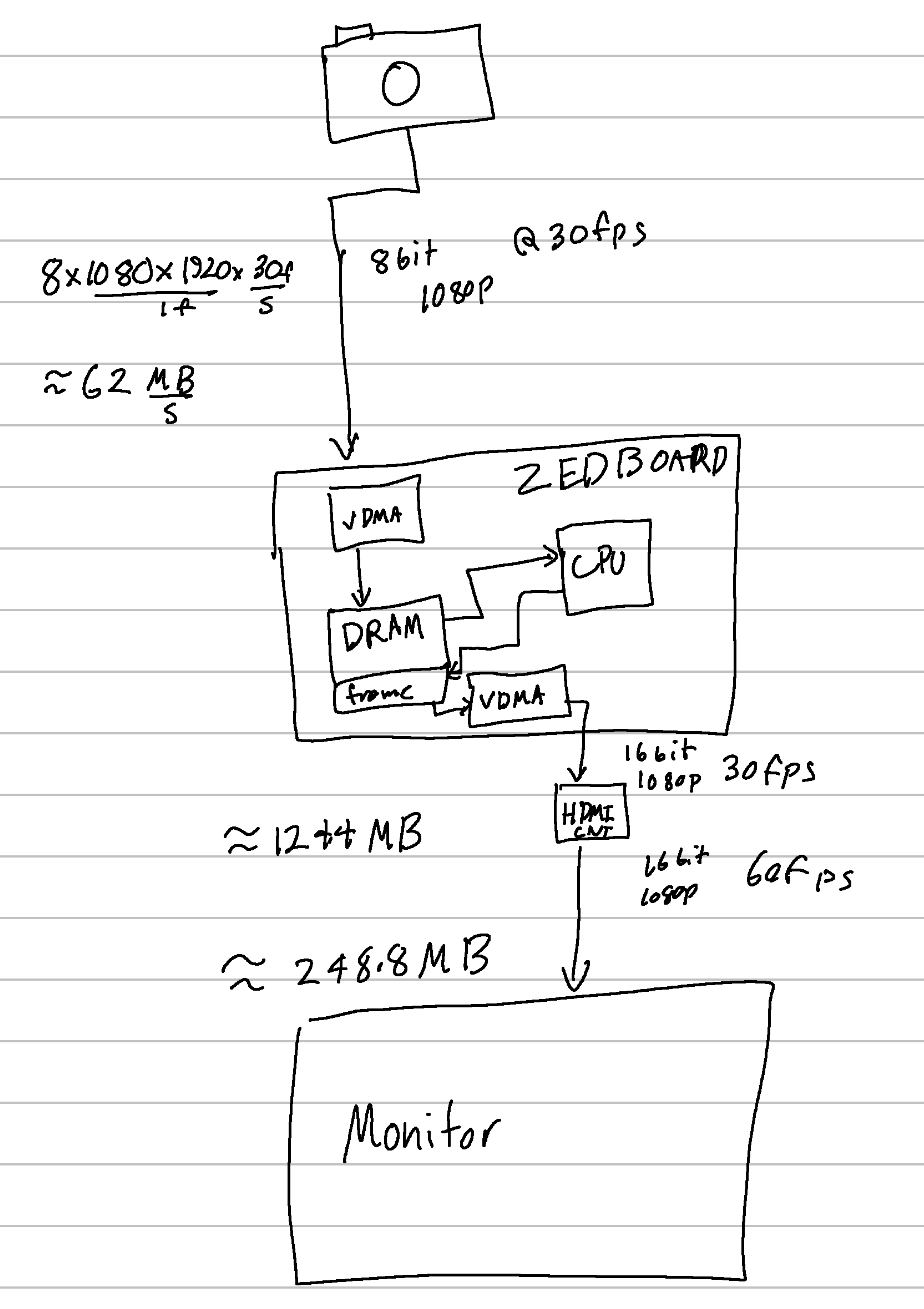
\includegraphics[width=4in]{images/Problem2-3.png} \\
\end{center}


Without compression or other optimization this data throughput would be much harder to achieve in embedded systems. Algorithms like the display stream compression can remove strain from lower level devices.\cite{Display Stream Compression}


\begin{thebibliography}{9}
\bibitem{Bayer Color}\href{https://kimon.hosting.nyu.edu/physical-electrical-digital/items/show/1083}{Bayer Color Filter Array}
\bibitem{Display Stream Compression}\href{https://en.wikipedia.org/wiki/Display_Stream_Compression}{Display Stream Compression}

\end{thebibliography}

\end{document}
